\chapter*{De Gujō à Kyoto\markboth{De Gujō à Kyoto}{}}
\section*{24 août 2015}
A une journée de vélo de Gujō j'arrive à Kakamigahara. Je reste une semaine en wwoofing chez Xavier et Yuka, un couple belge/japonais. \newline
 \newline
\centerline{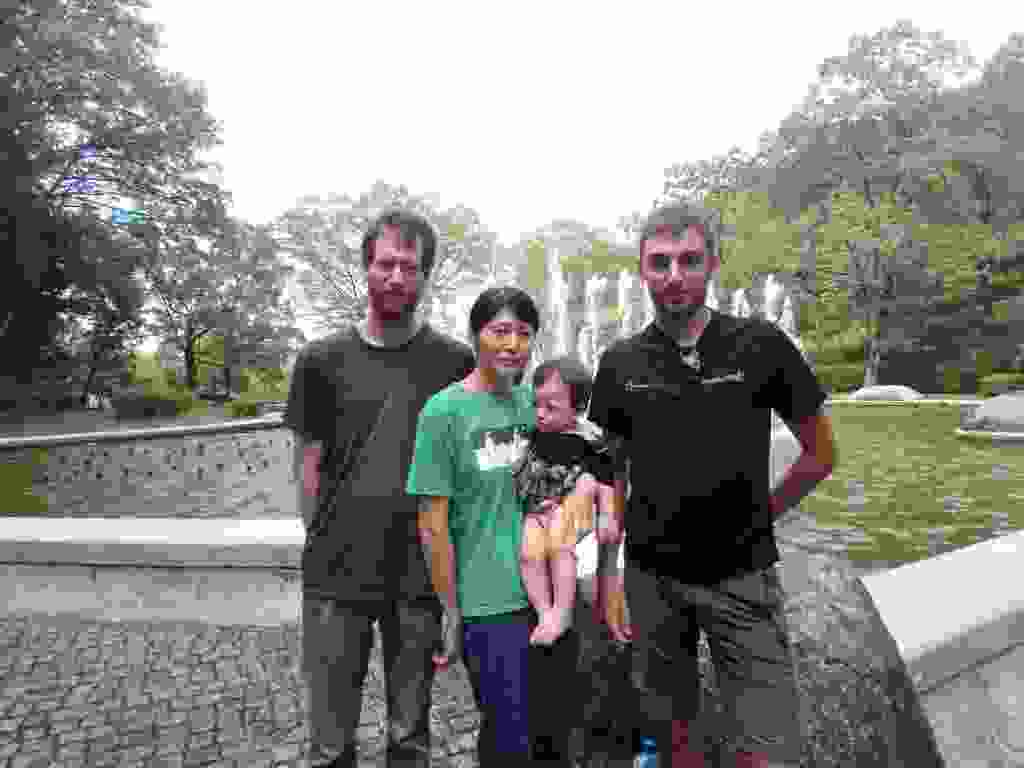
\includegraphics[width=\mywidth]{../wp-content/uploads/2015/08/P8166185-1024x768.jpg} } 
 \newline
 Le principe du wwoofing est d'aider dans une ferme en échange du gite et du couvert. \newline
 Xavier a plusieurs rizières et un champ en maraichage. Il expérimente les principes de l'agriculture naturelle, technique issue du Japon. \newline
 \newline
\centerline{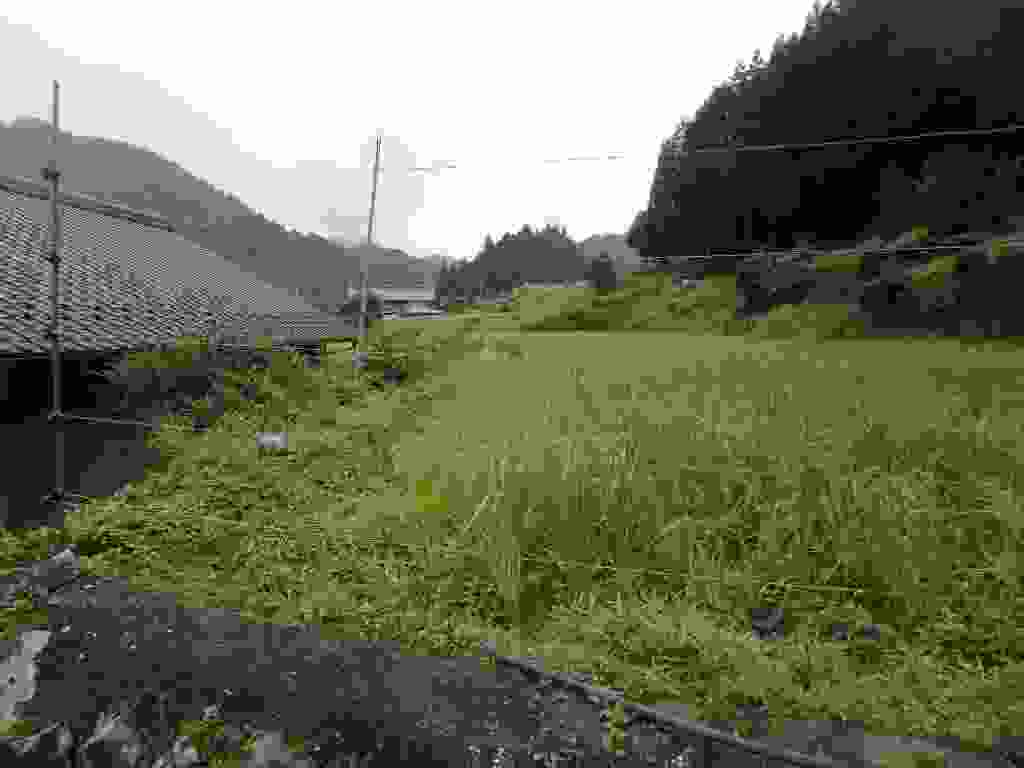
\includegraphics[width=\mywidth]{../wp-content/uploads/2015/08/P8146136-1024x768.jpg} } 
 \newline
 \newline
\centerline{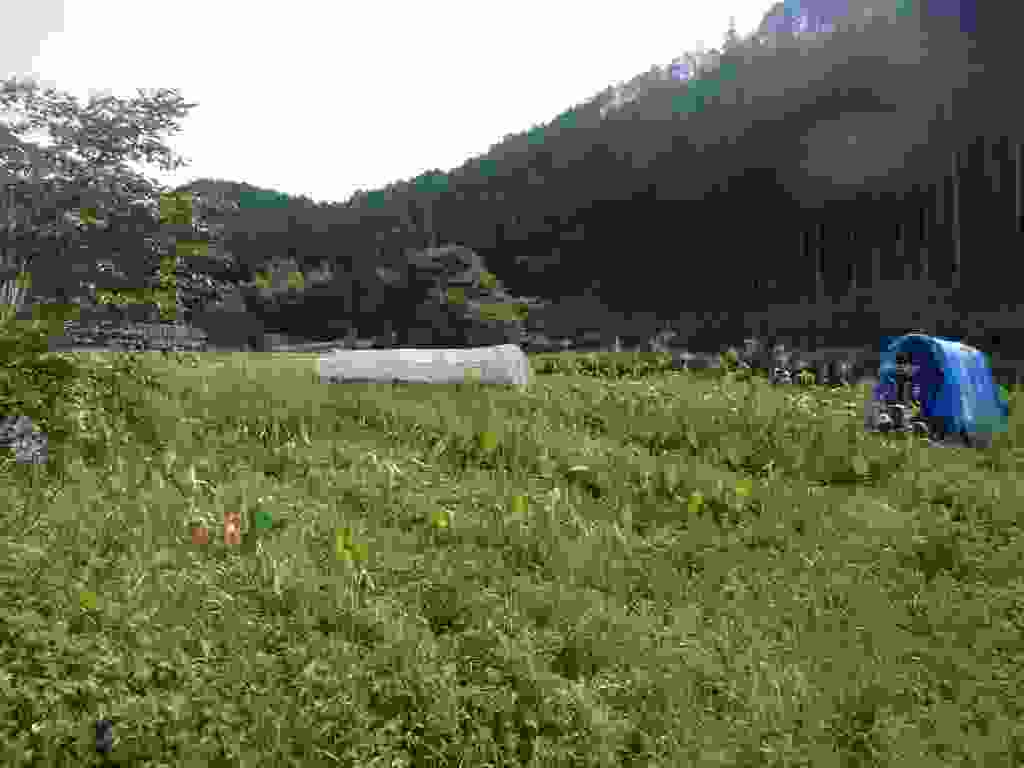
\includegraphics[width=\mywidth]{../wp-content/uploads/2015/08/P8116128-1024x768.jpg} } 
 \newline
 Kakamigahara est le centre de l'aéronautique au Japon, un musée y est consacré \newline
 \newline
\centerline{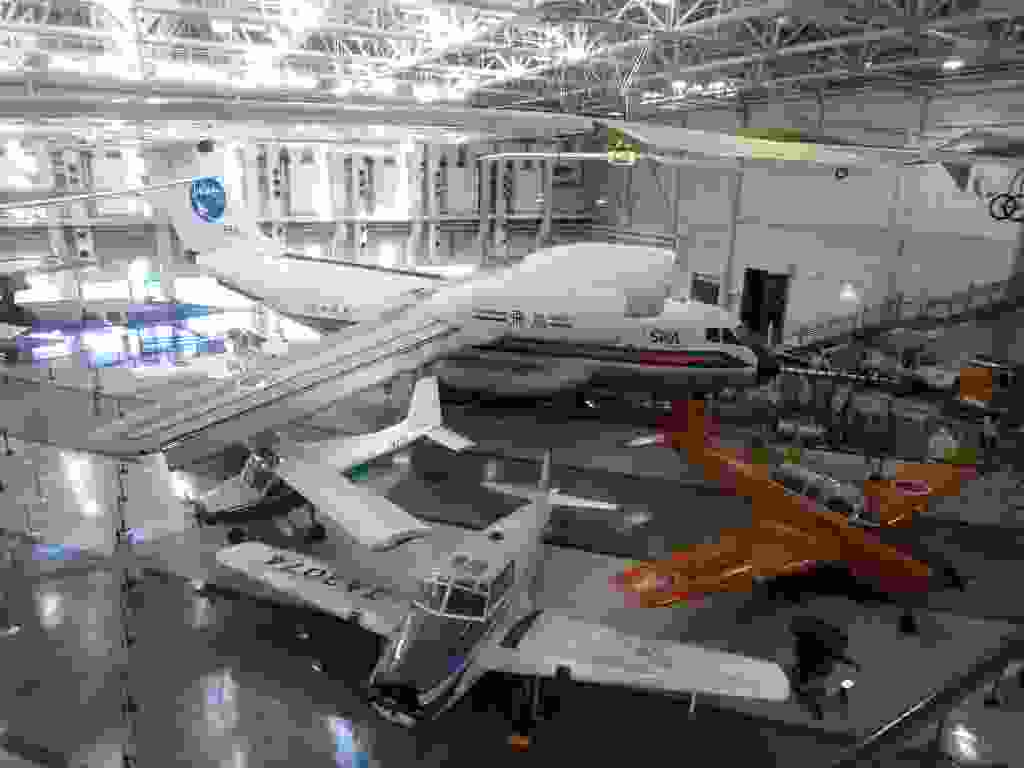
\includegraphics[width=\mywidth]{../wp-content/uploads/2015/08/P8156175-1024x768.jpg} } 
 \newline
 \newline
\centerline{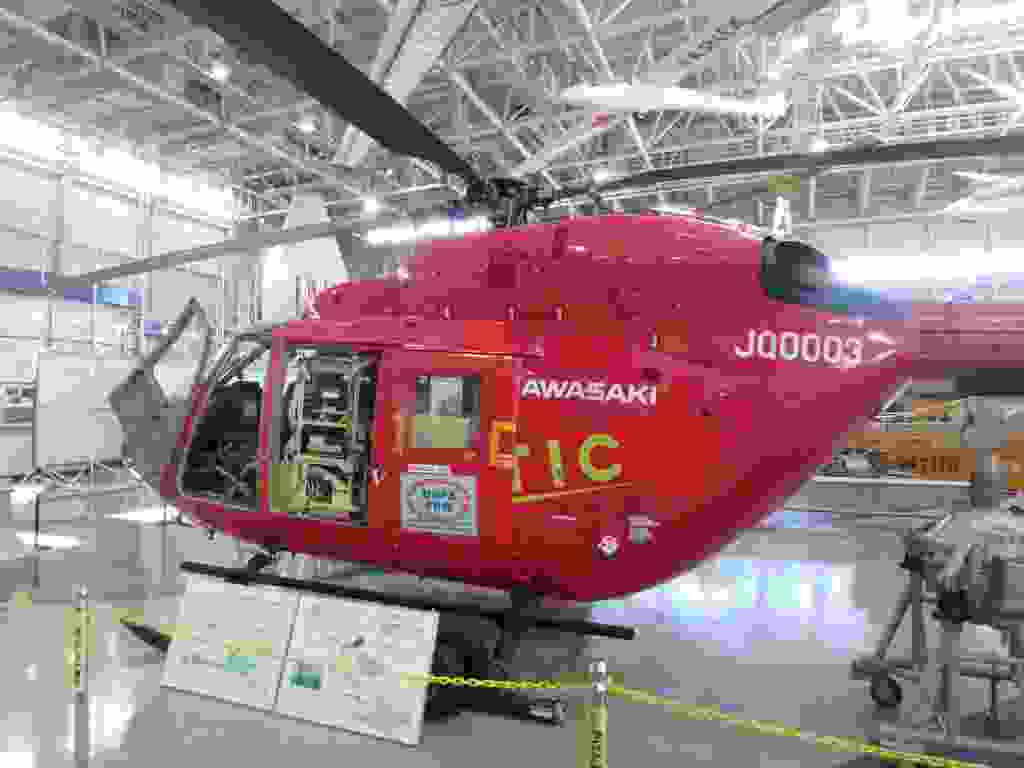
\includegraphics[width=\mywidth]{../wp-content/uploads/2015/08/P8156173-1024x768.jpg} } 
 \newline
 A coté la ville d'Inuyama : son célèbre château \newline
 \newline
\centerline{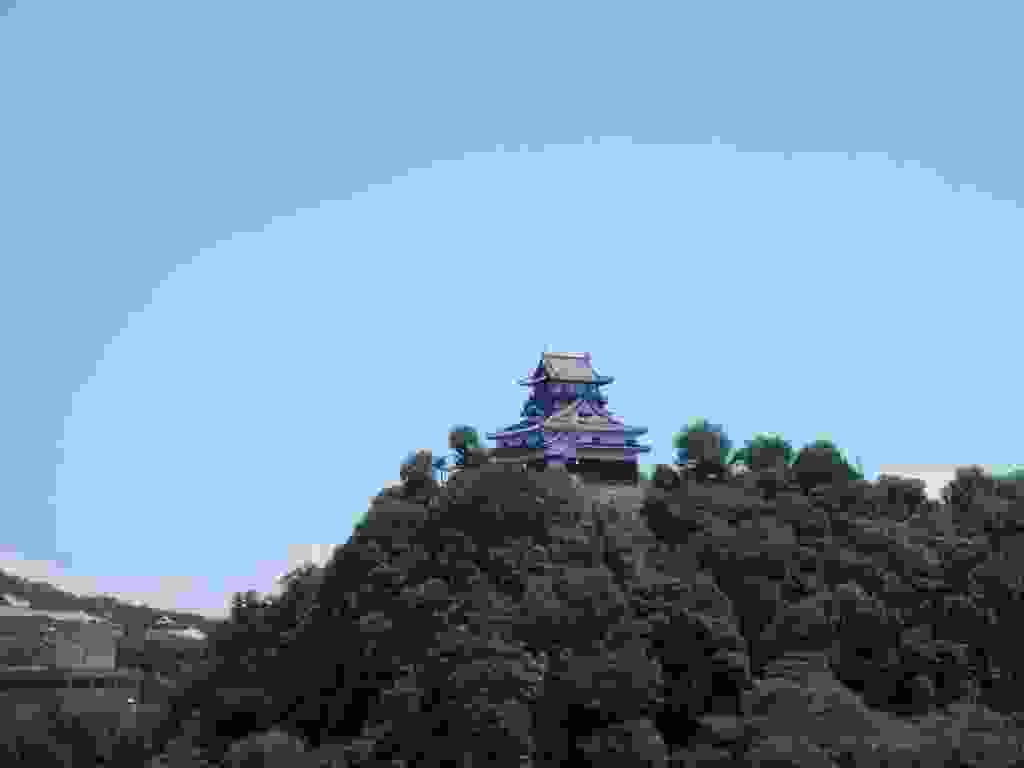
\includegraphics[width=\mywidth]{../wp-content/uploads/2015/08/P8156139-1024x768.jpg} } 
 \newline
 \newline
\centerline{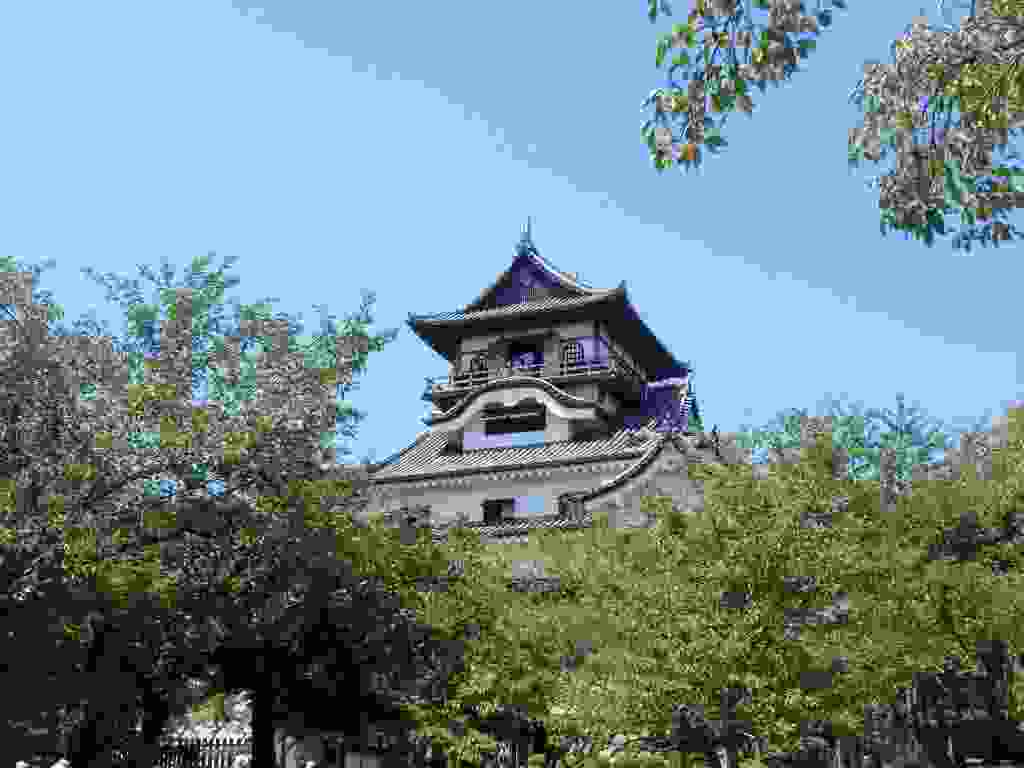
\includegraphics[width=\mywidth]{../wp-content/uploads/2015/08/P8156148-1024x768.jpg} } 
 \newline
 Le jardin Jo-an avec des maisons de thé \newline
 \newline
\centerline{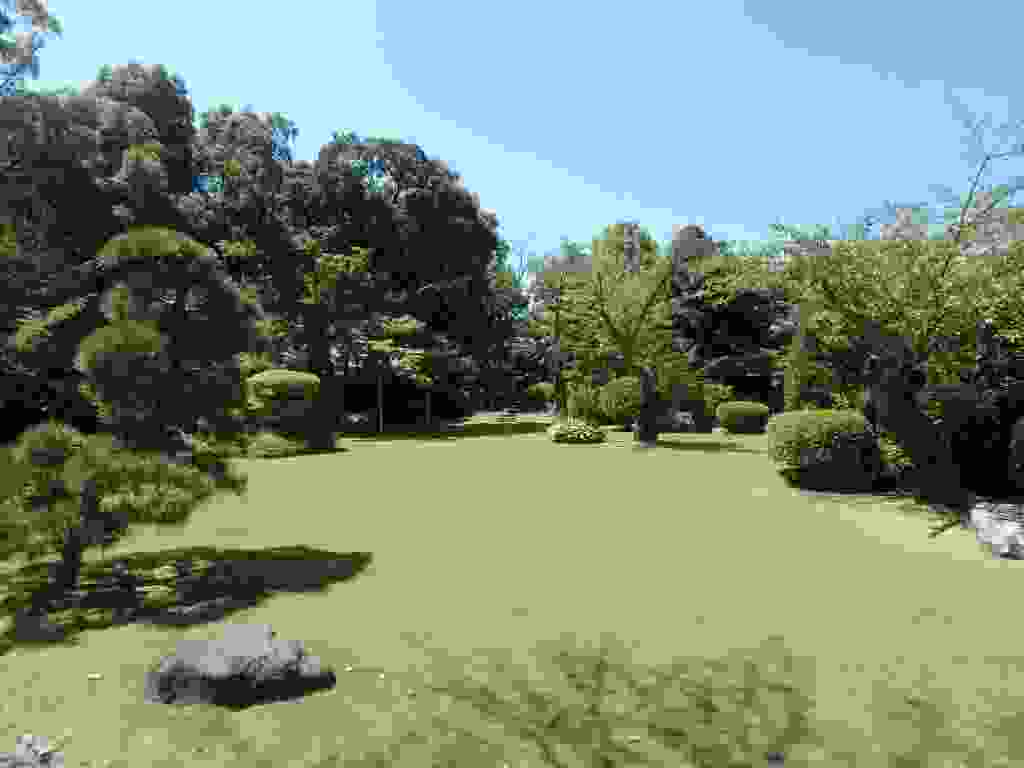
\includegraphics[width=\mywidth]{../wp-content/uploads/2015/08/P8156150-1024x768.jpg} } 
 \newline
 \newline
\centerline{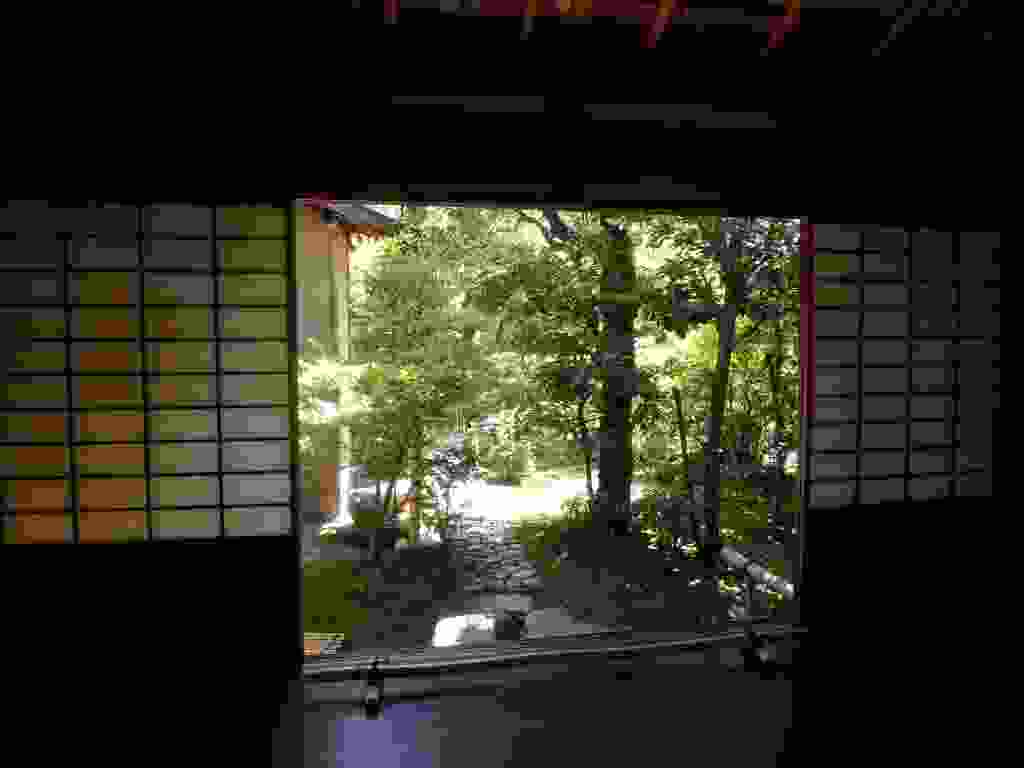
\includegraphics[width=\mywidth]{../wp-content/uploads/2015/08/P8156149-1024x768.jpg} } 
 \newline
 \newline
\centerline{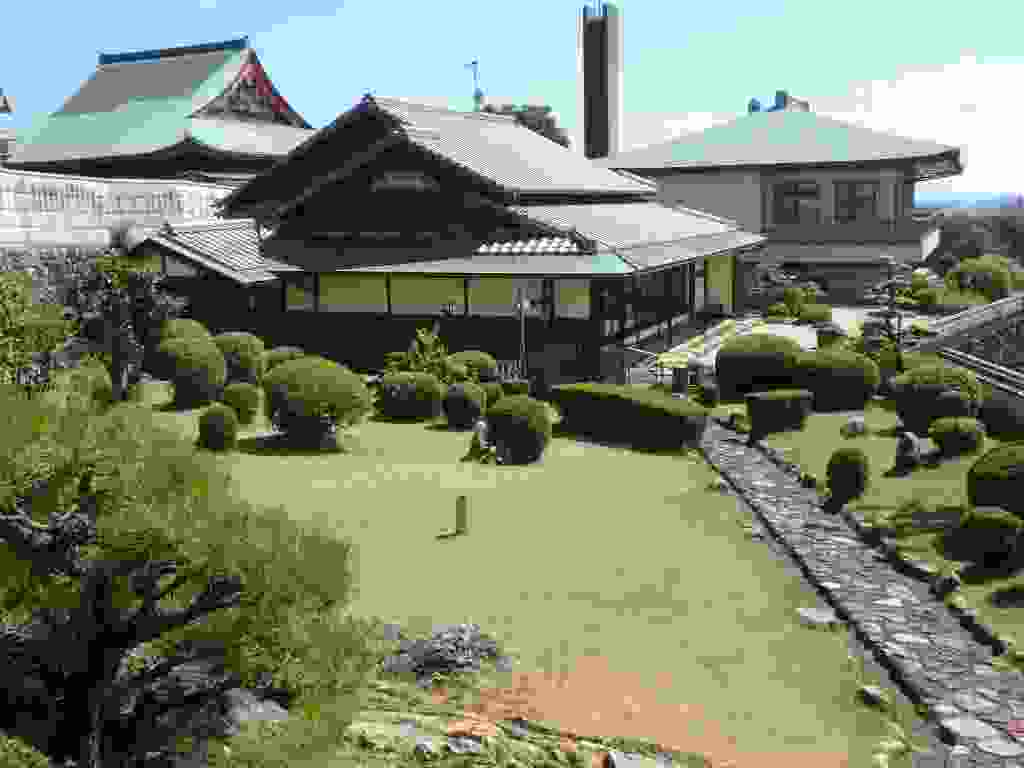
\includegraphics[width=\mywidth]{../wp-content/uploads/2015/08/P8156167-1024x768.jpg} } 
 \newline
 Le temple de Zuizen-ji \newline
 \newline
\centerline{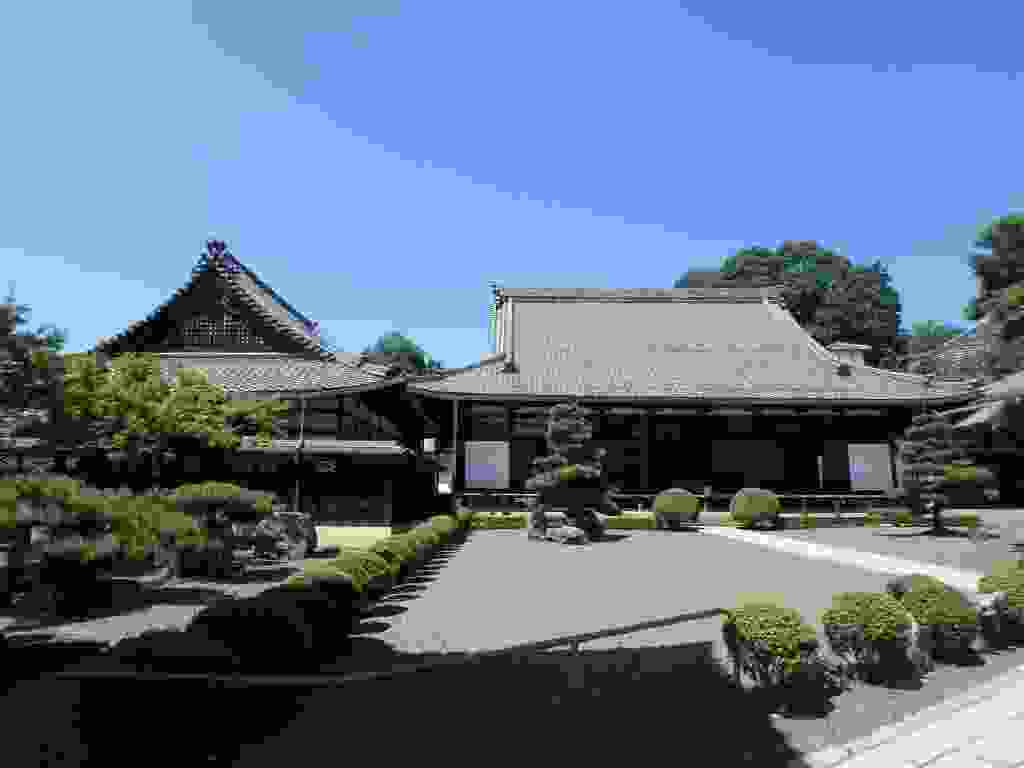
\includegraphics[width=\mywidth]{../wp-content/uploads/2015/08/P8156154-1024x768.jpg} } 
 \newline
 A Gifu, j'assiste au spectacle nocturne de la pêche aux cormorans. \newline
 \newline
\centerline{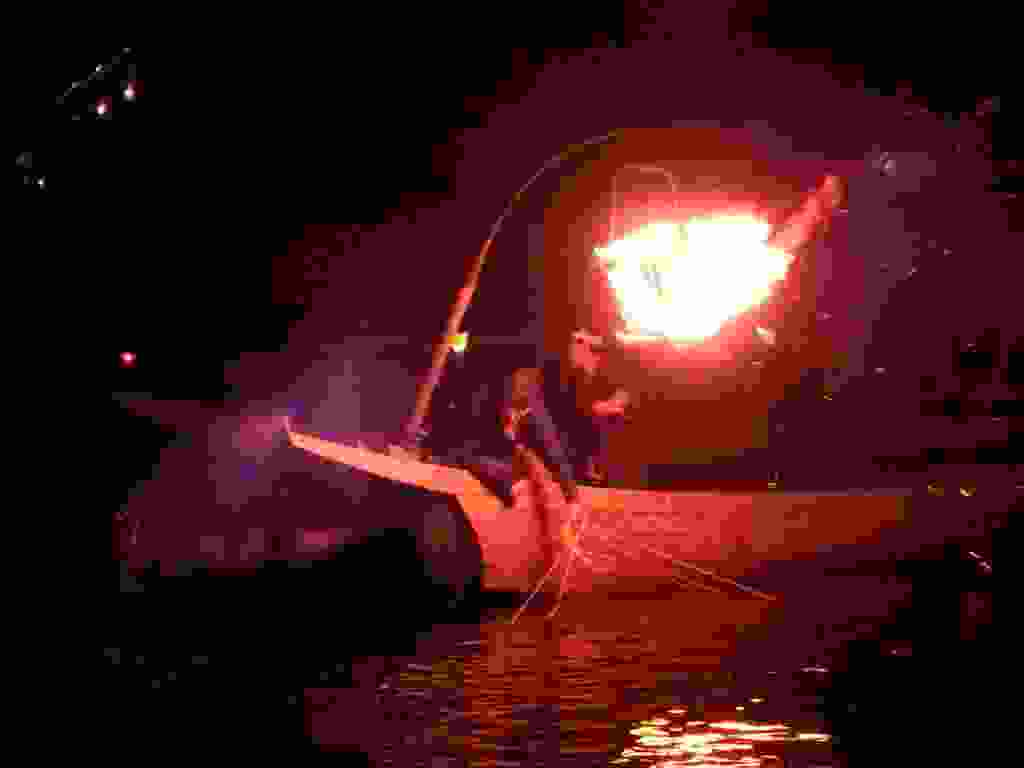
\includegraphics[width=\mywidth]{../wp-content/uploads/2015/08/P8166194-1024x768.jpg} } 
 \newline
 \newline
\centerline{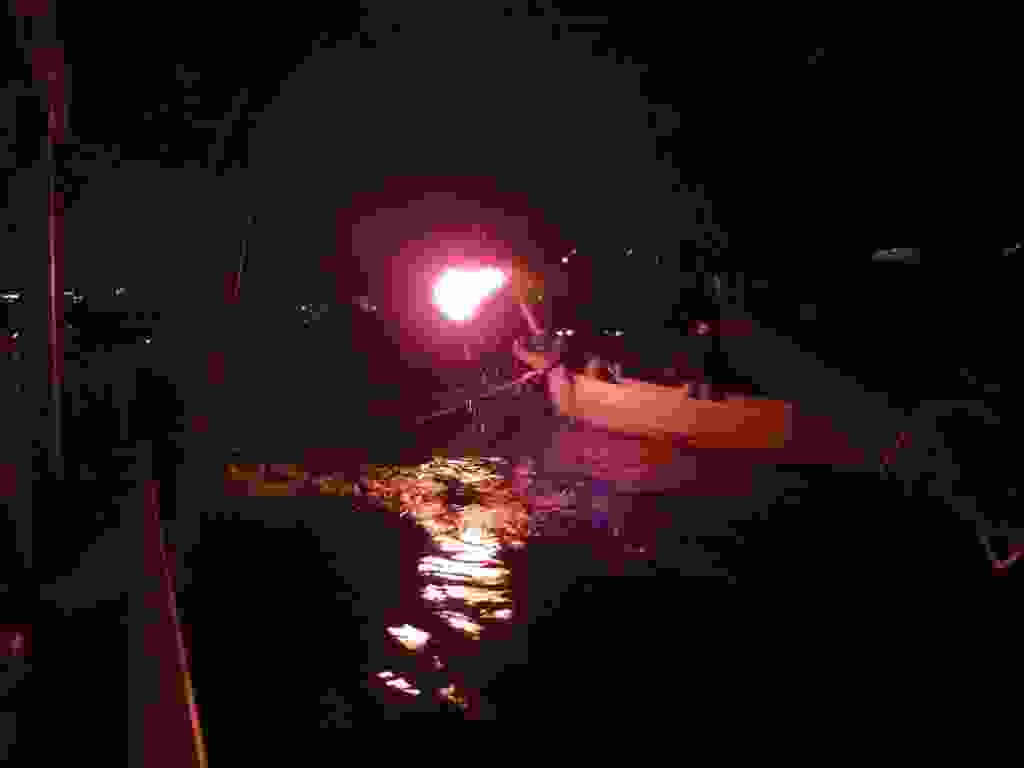
\includegraphics[width=\mywidth]{../wp-content/uploads/2015/08/P8166195-1024x768.jpg} } 
 \newline
 \newline
\centerline{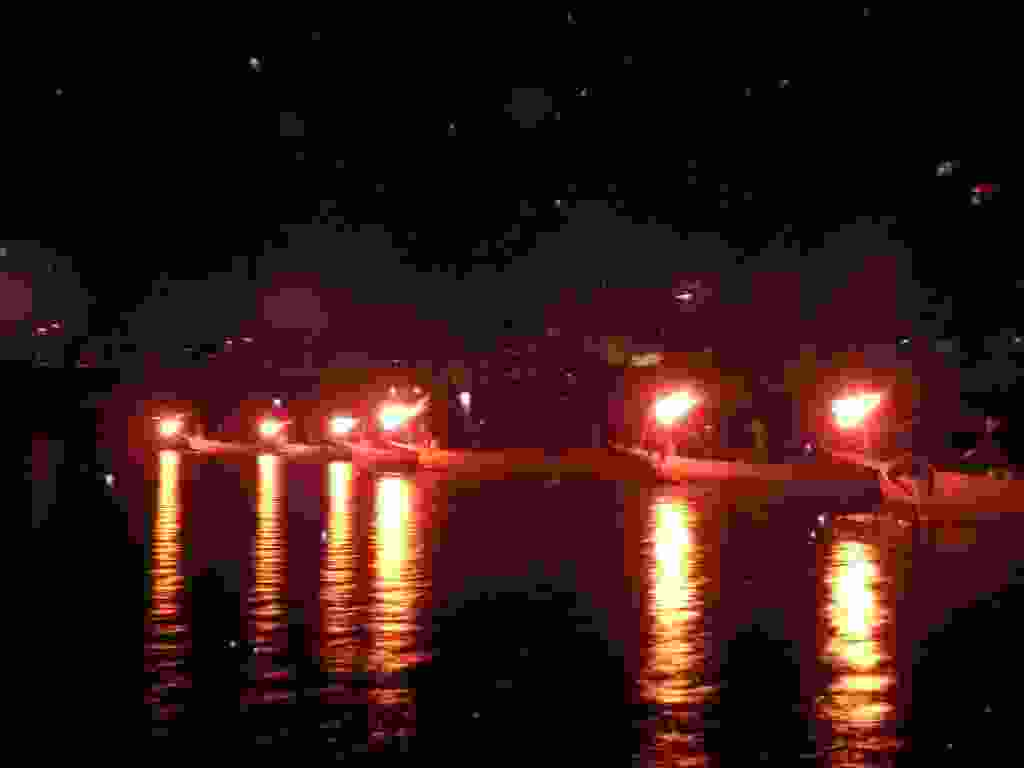
\includegraphics[width=\mywidth]{../wp-content/uploads/2015/08/P8166200-1024x768.jpg} } 
 \newline
 Je repars en direction de Kyoto et je m'arrête au château d'Hikone \newline
 \newline
\centerline{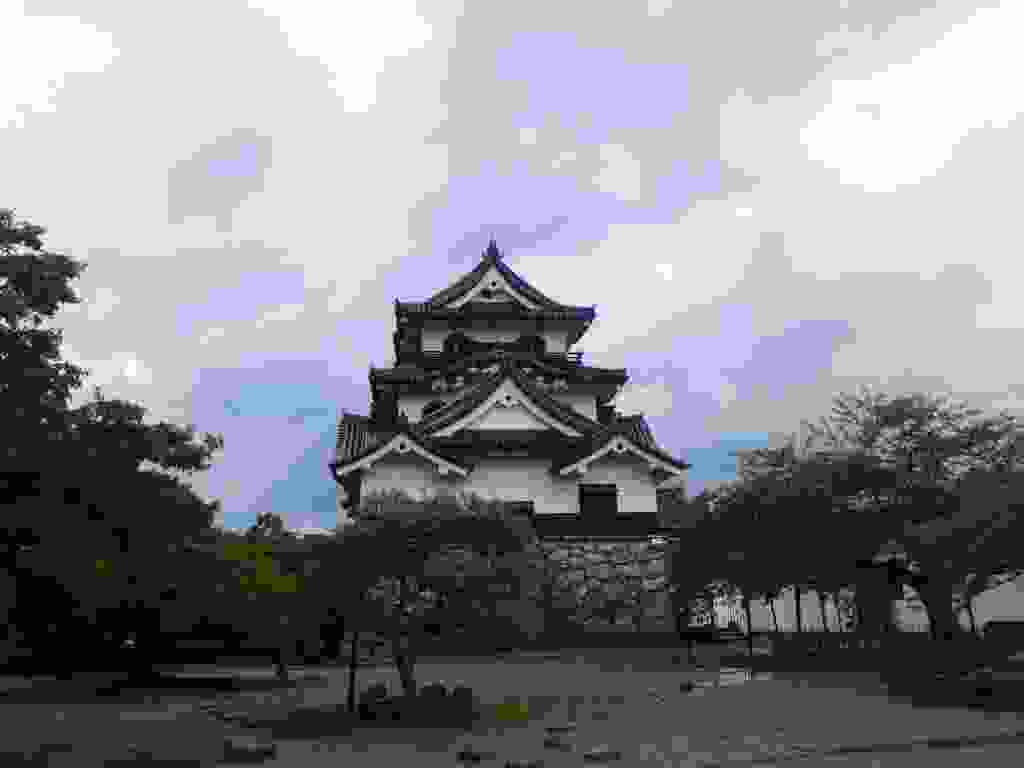
\includegraphics[width=\mywidth]{../wp-content/uploads/2015/08/P8176204-1024x768.jpg} } 
 \newline
 Beau jardin en contrebas du château \newline
 \newline
\centerline{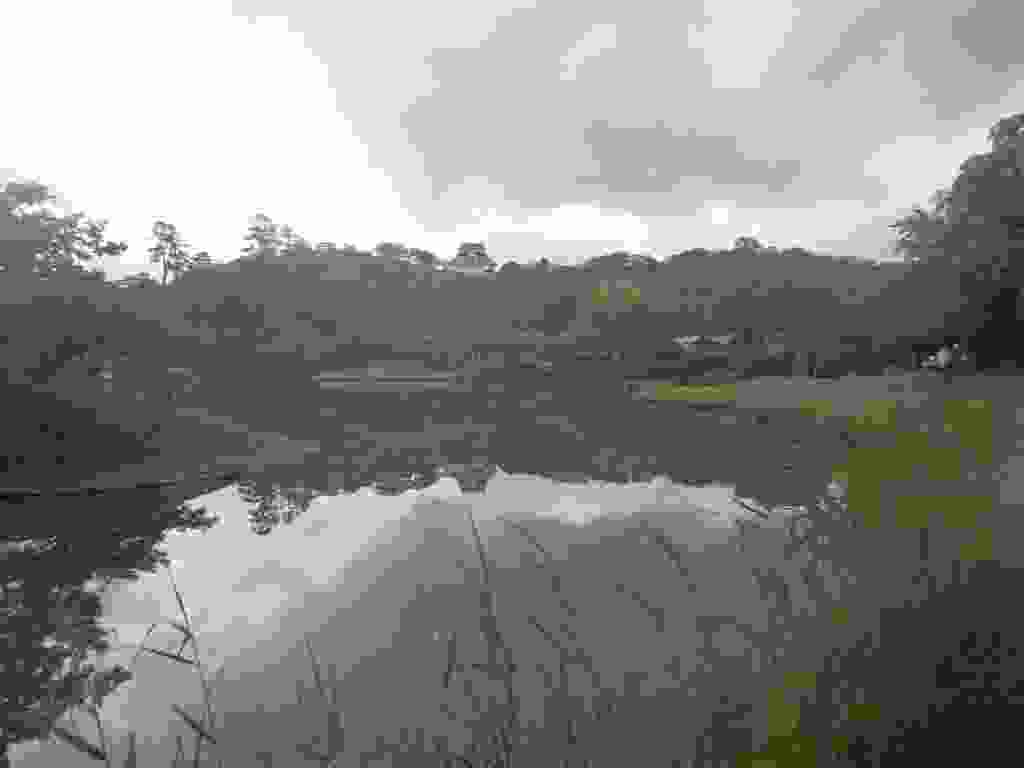
\includegraphics[width=\mywidth]{../wp-content/uploads/2015/08/P8176214-1024x768.jpg} } 
 \newline
 \newline
\centerline{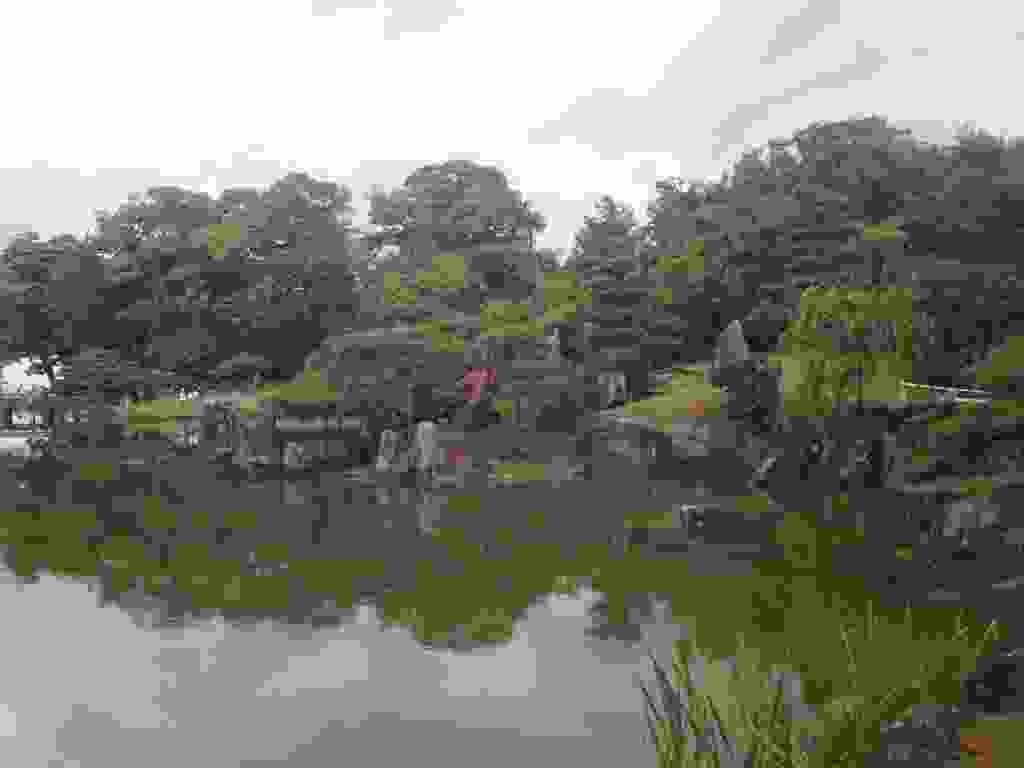
\includegraphics[width=\mywidth]{../wp-content/uploads/2015/08/P8176217-1024x768.jpg} } 
 \newline
 Je longe ensuite le lac Biwa, le plus grand du Japon \newline
 \newline
\centerline{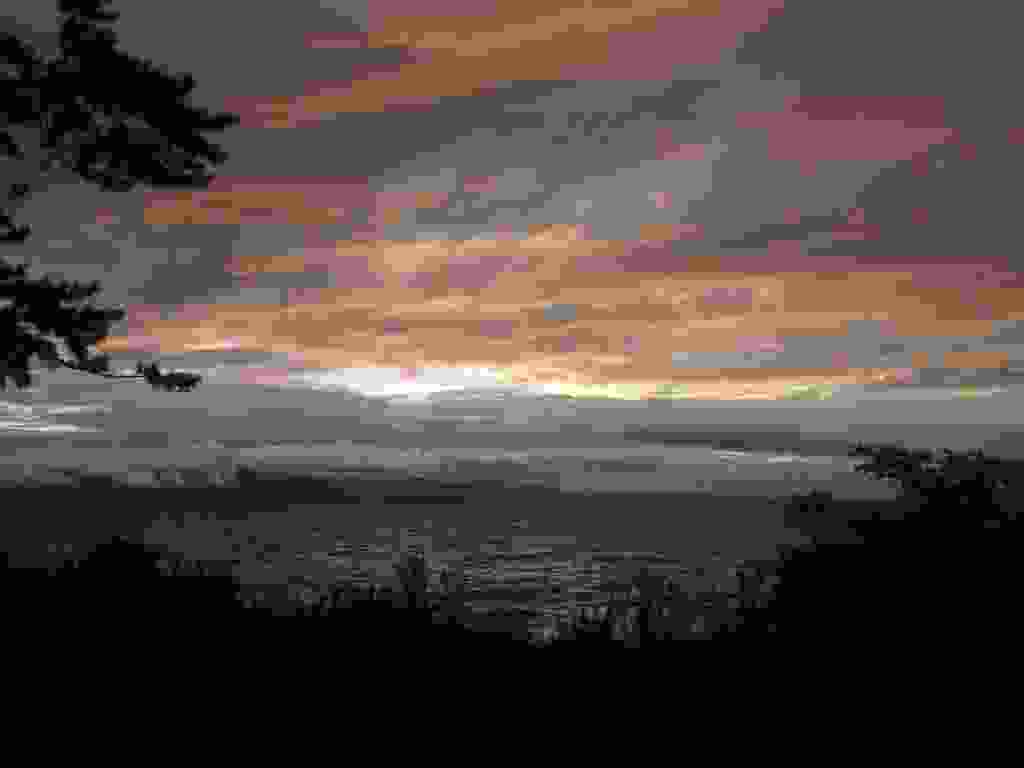
\includegraphics[width=\mywidth]{../wp-content/uploads/2015/08/P8176222-1024x768.jpg} } 
 \newline
 \newline
\centerline{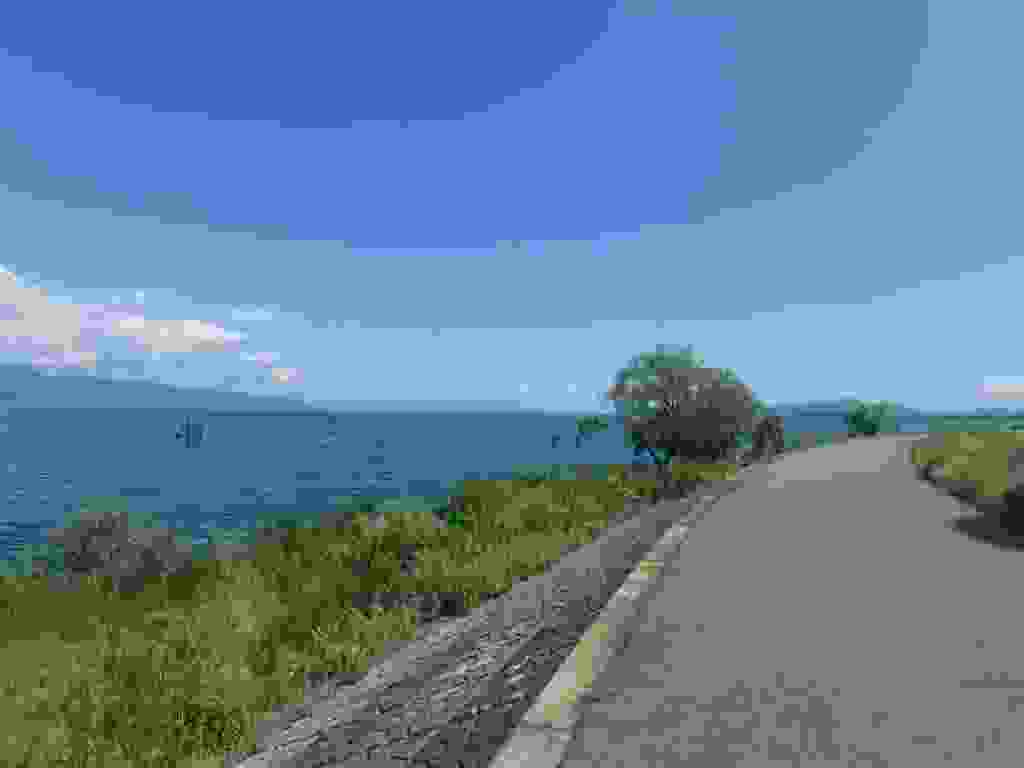
\includegraphics[width=\mywidth]{../wp-content/uploads/2015/08/P8186228-1024x768.jpg} } 
 \newline
 \newline
\centerline{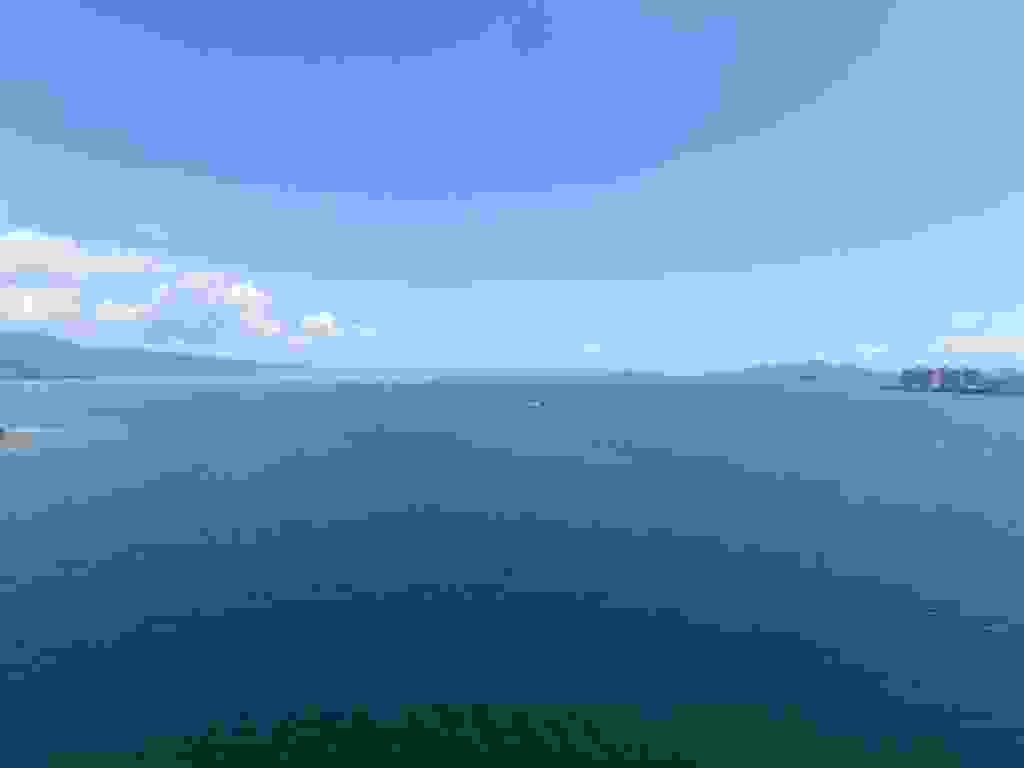
\includegraphics[width=\mywidth]{../wp-content/uploads/2015/08/P8186229-1024x768.jpg} } 
 \newline
 Quelques km avant Kyoto, arrêt pour visiter 2 temples \newline
 \newline
\centerline{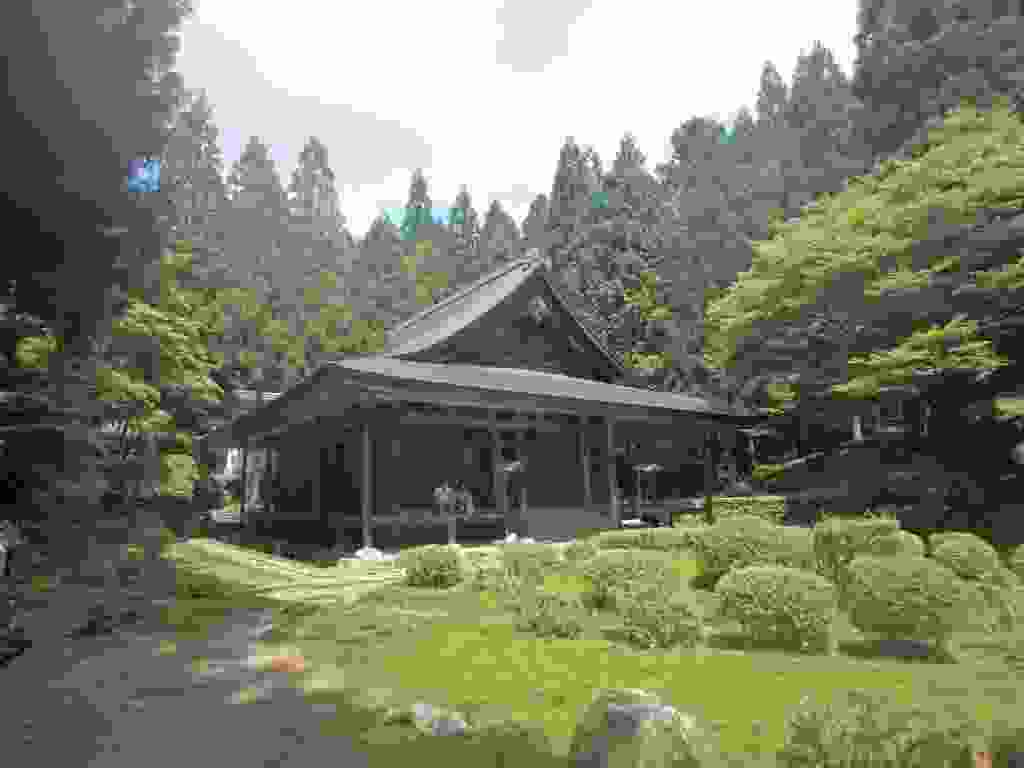
\includegraphics[width=\mywidth]{../wp-content/uploads/2015/08/P8186232-1024x768.jpg} } 
 \newline
 \newline
\centerline{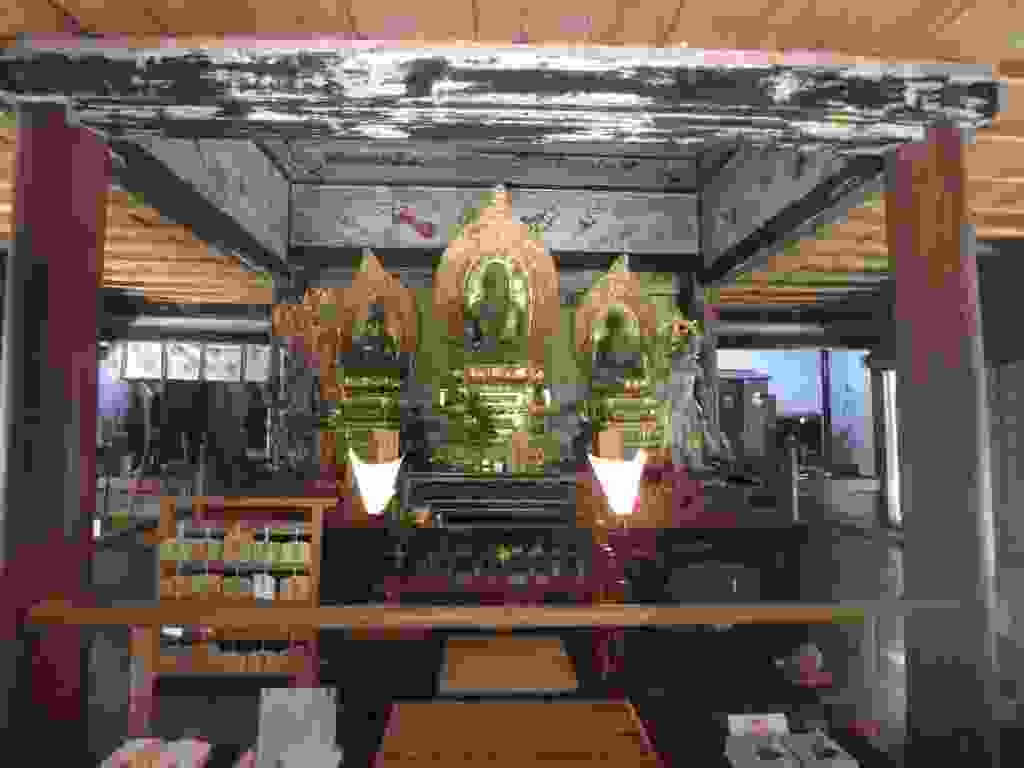
\includegraphics[width=\mywidth]{../wp-content/uploads/2015/08/P8186233-1024x768.jpg} } 
 \newline
 \newline
\centerline{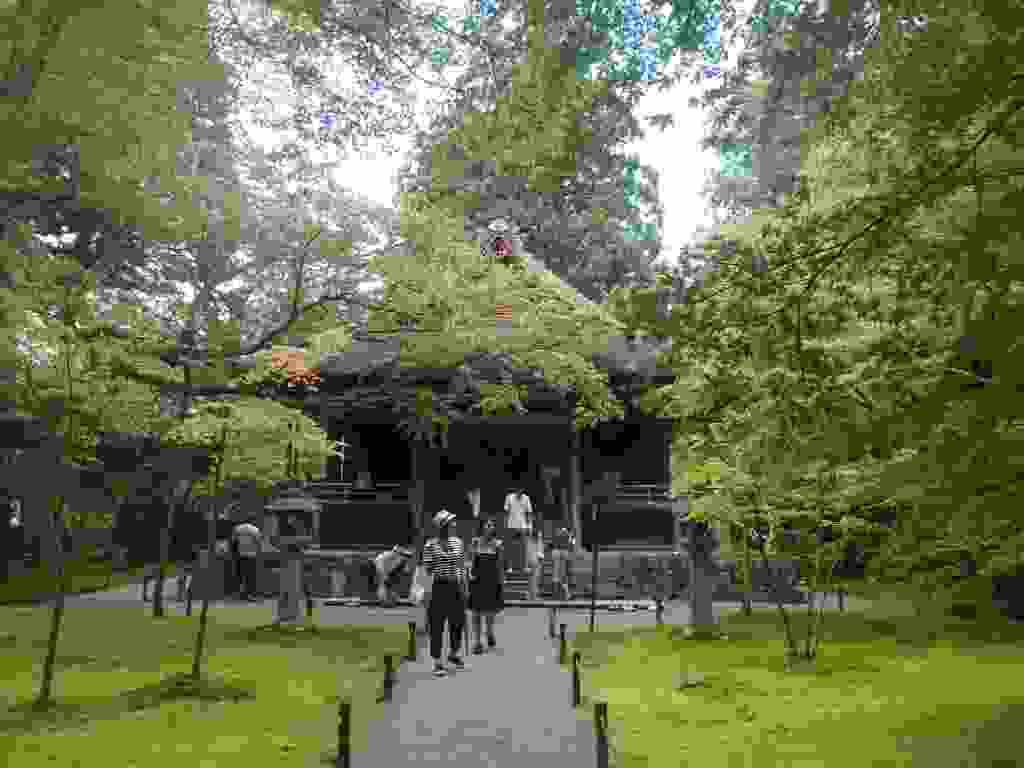
\includegraphics[width=\mywidth]{../wp-content/uploads/2015/08/P8186243-1024x768.jpg} } 
 \newline
 \newline
\centerline{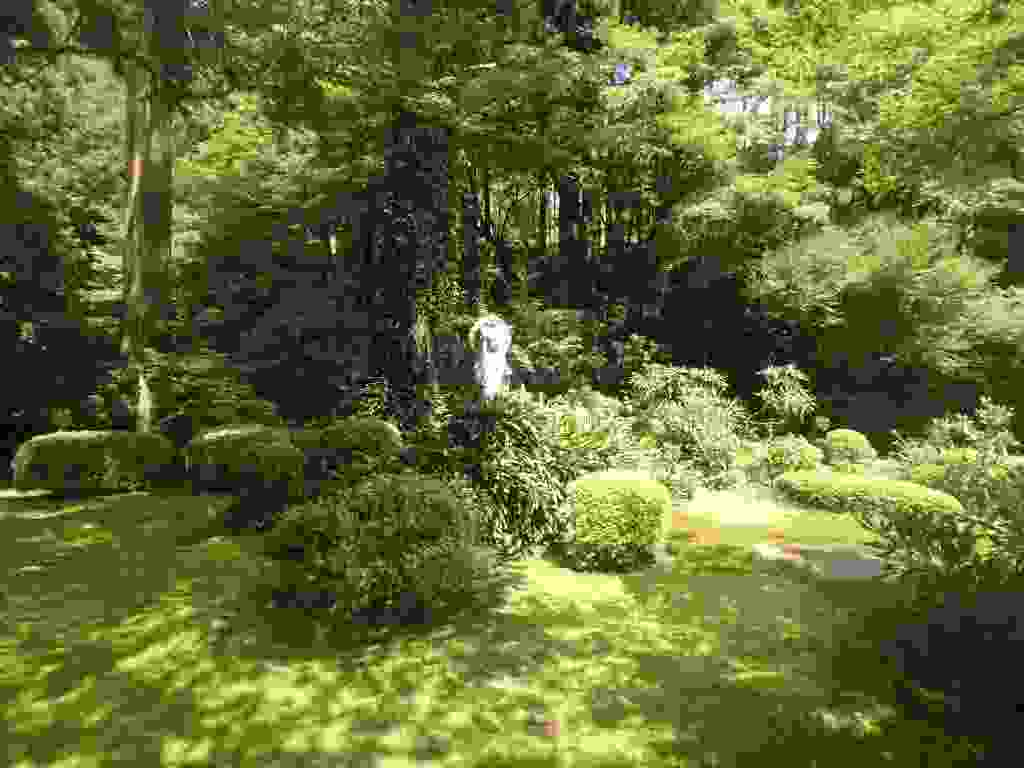
\includegraphics[width=\mywidth]{../wp-content/uploads/2015/08/P8186241-1024x768.jpg} } 
 \newline
 A Kyoto je suis recu par Ken qui est malaisien. \newline
 Il m'emmène gouter un okonomiyaki, galette à base de chou complétée par viande, fromage ou oeuf selon les versions. \newline
 \newline
\centerline{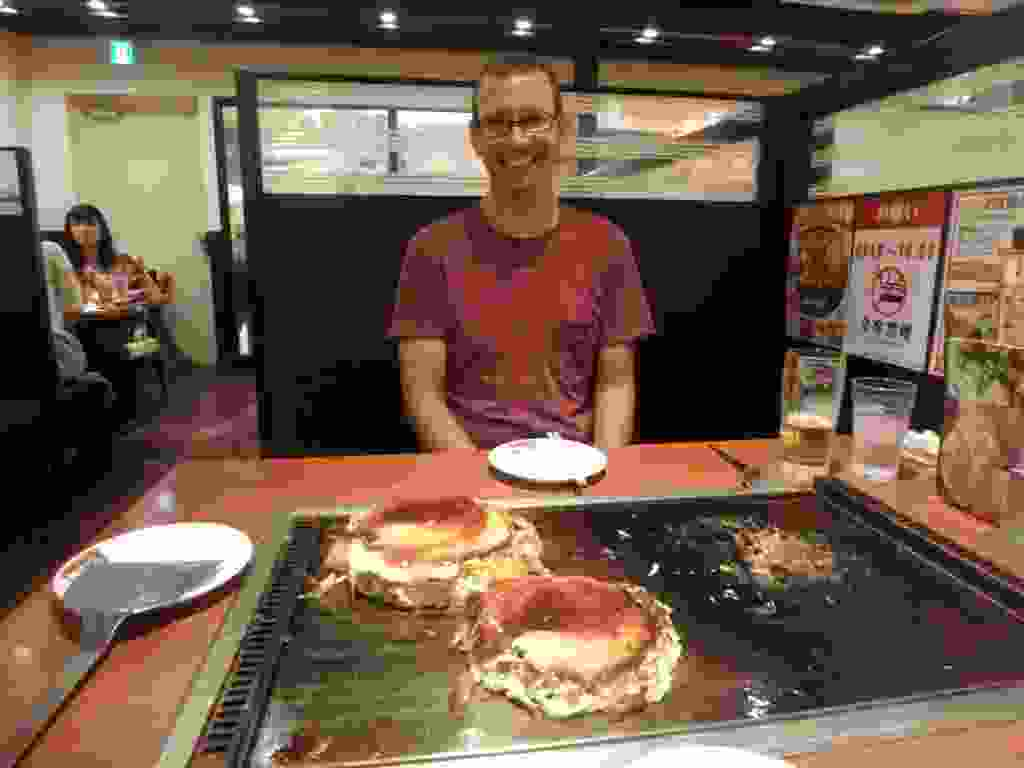
\includegraphics[width=\mywidth]{../wp-content/uploads/2015/08/P8196331-1024x768.jpg} } 
 \newline
 Grace à lui je rencontre Bruce et Chiara, un couple de cyclistes américains en vélos pliants \newline
 \newline
\centerline{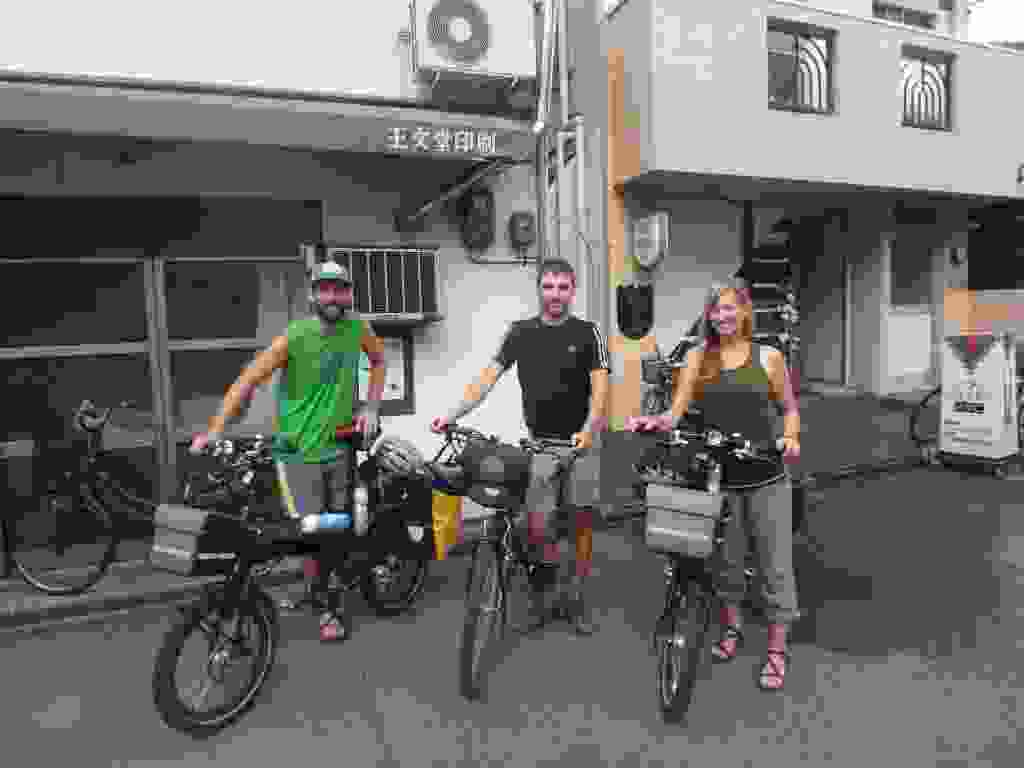
\includegraphics[width=\mywidth]{../wp-content/uploads/2015/08/P8196253-1024x768.jpg} } 
 \newline
 Il y a des centaines de temples et shrines à Kyoto, je suis allé en voir quelques uns. \newline
 Shrine Fushimi Inari-taisha et ses milliers de portes \newline
 \newline
\centerline{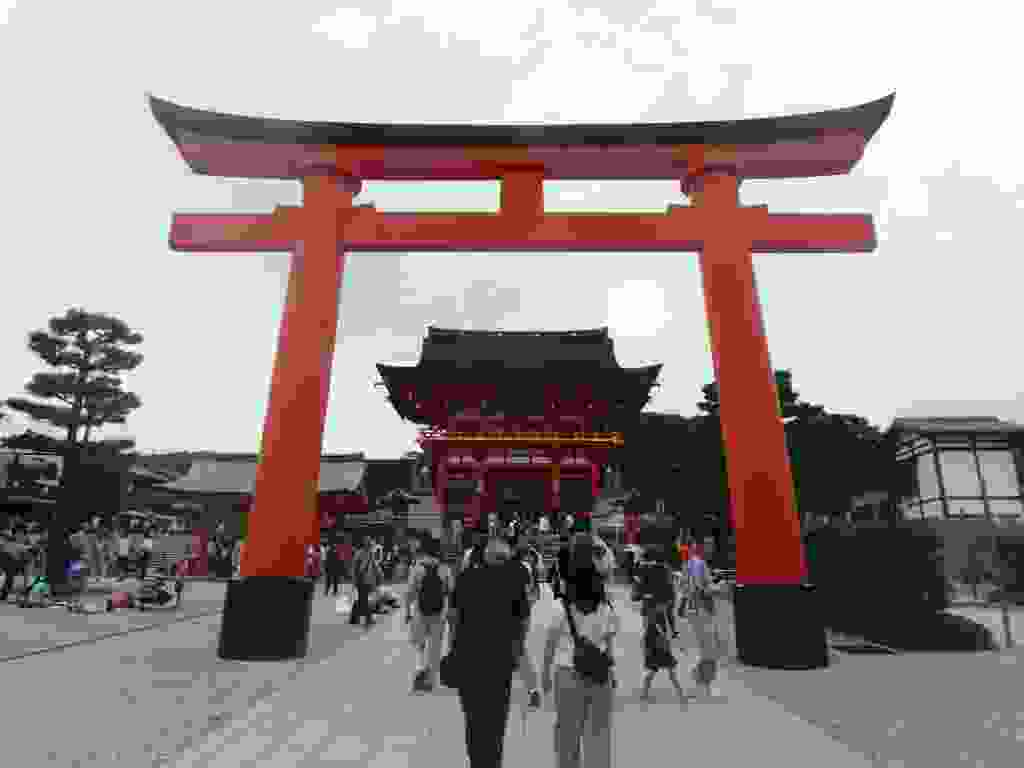
\includegraphics[width=\mywidth]{../wp-content/uploads/2015/08/P8196254-1024x768.jpg} } 
 \newline
 \newline
\centerline{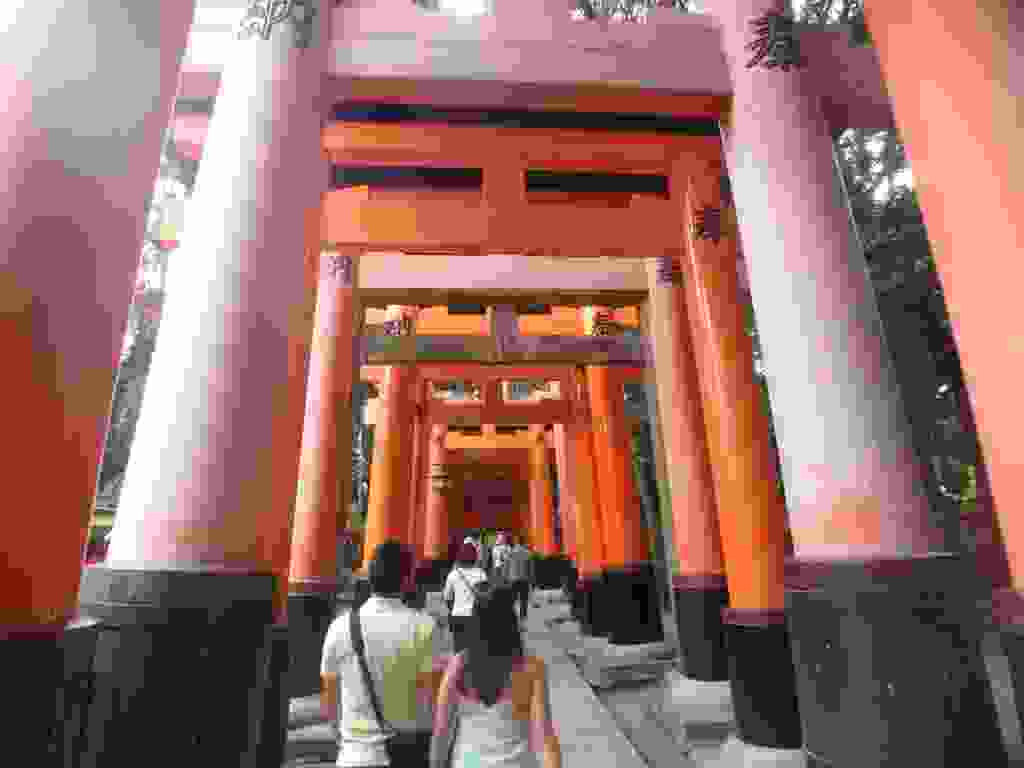
\includegraphics[width=\mywidth]{../wp-content/uploads/2015/08/P8196257-1024x768.jpg} } 
 \newline
 \newline
\centerline{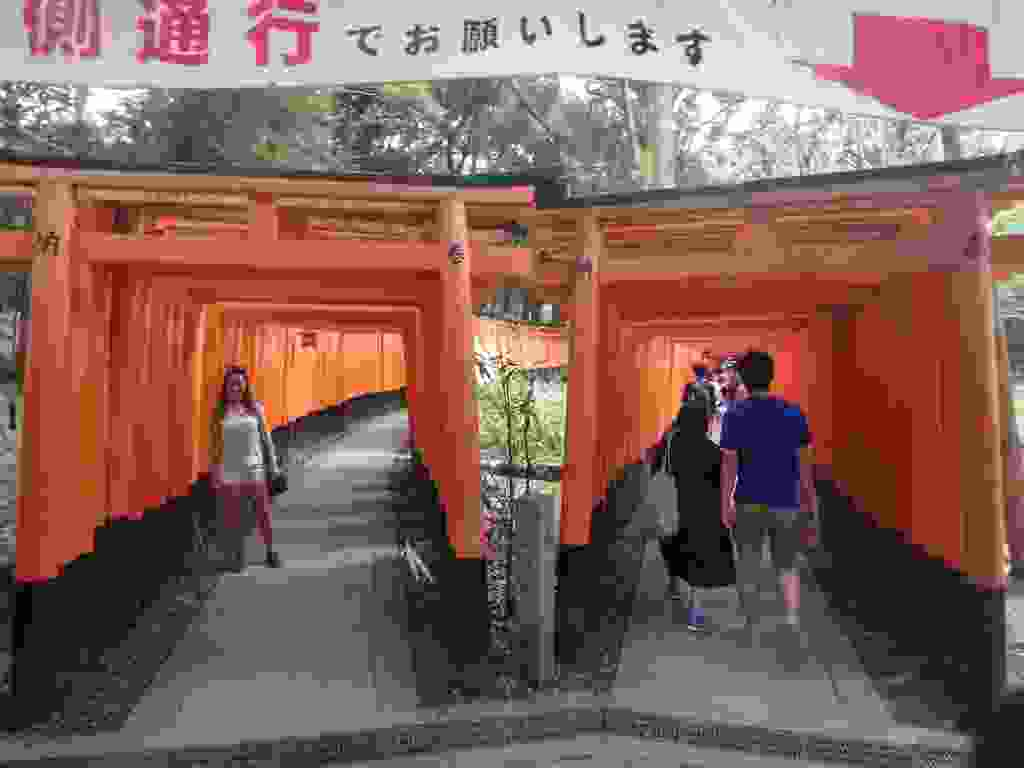
\includegraphics[width=\mywidth]{../wp-content/uploads/2015/08/P8196259-1024x768.jpg} } 
 \newline
 Shrine Shimogamo, un des plus anciens du Japon \newline
 \newline
\centerline{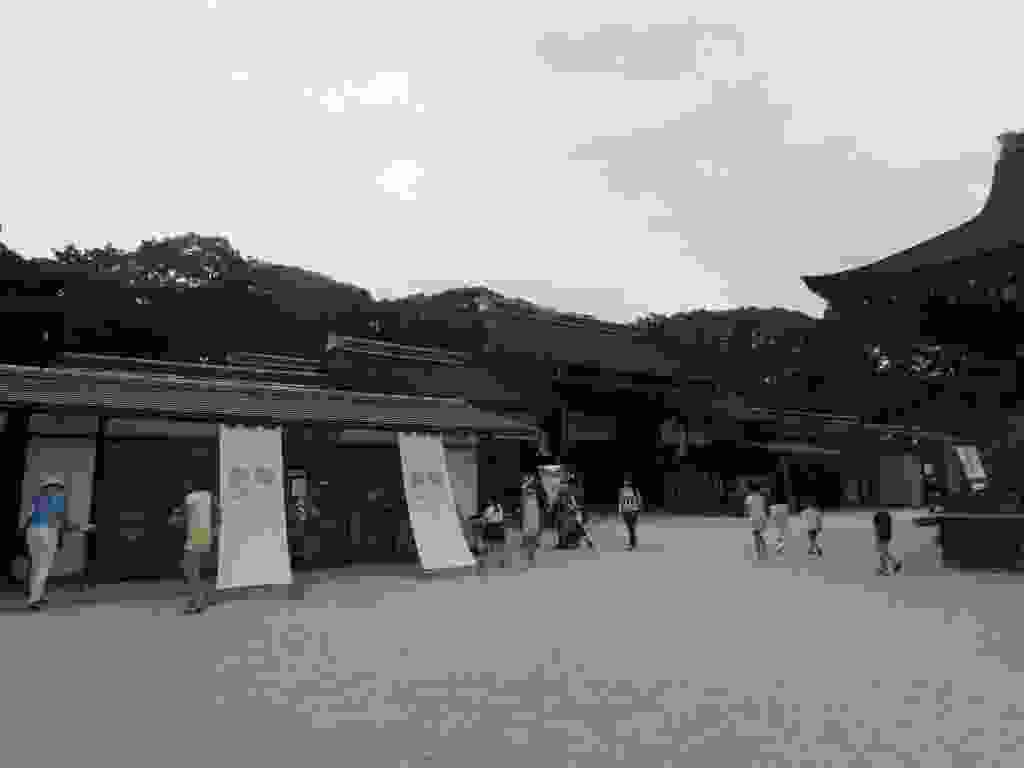
\includegraphics[width=\mywidth]{../wp-content/uploads/2015/08/P8196267-1024x768.jpg} } 
 \newline
 Ginkaku-ji, le pavillon d'argent \newline
 \newline
\centerline{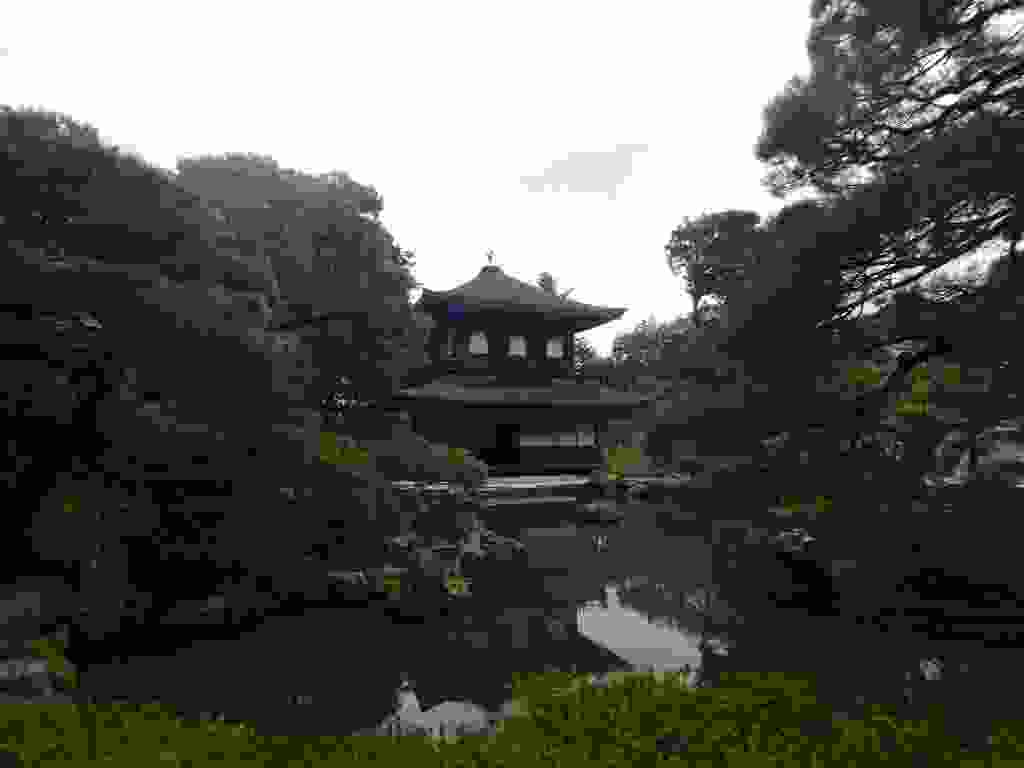
\includegraphics[width=\mywidth]{../wp-content/uploads/2015/08/P8196284-1024x768.jpg} } 
 \newline
 \newline
\centerline{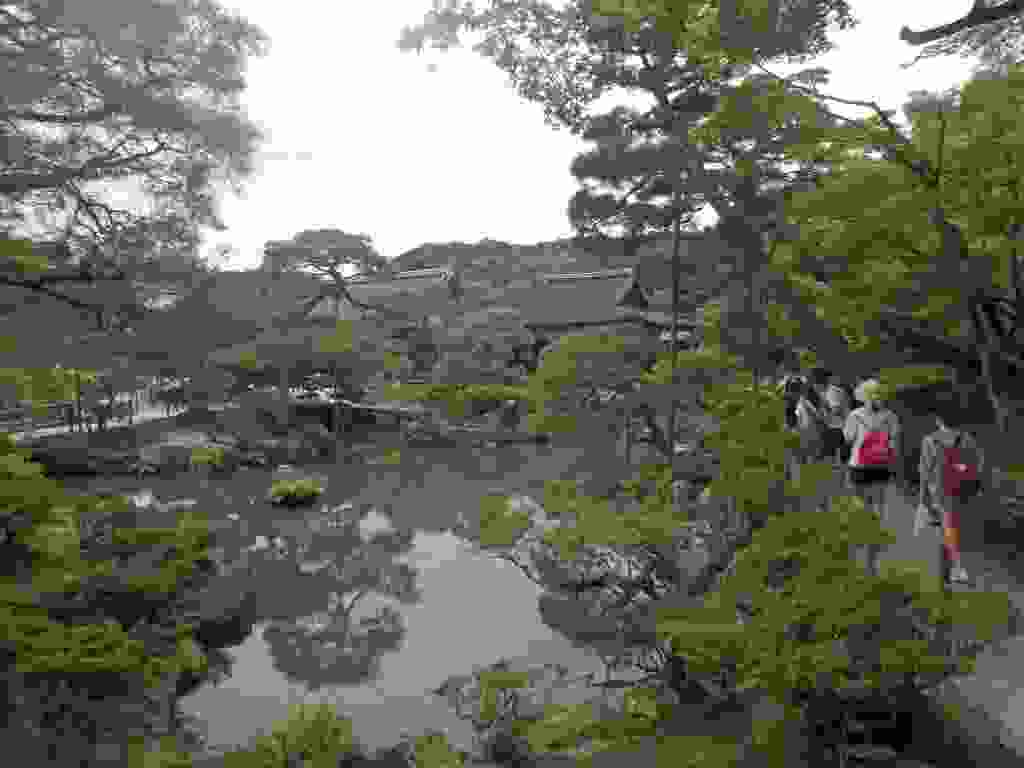
\includegraphics[width=\mywidth]{../wp-content/uploads/2015/08/P8196278-1024x768.jpg} } 
 \newline
 Temple Kiyomizu-dera, peut être le plus visité de Kyoto \newline
 \newline
\centerline{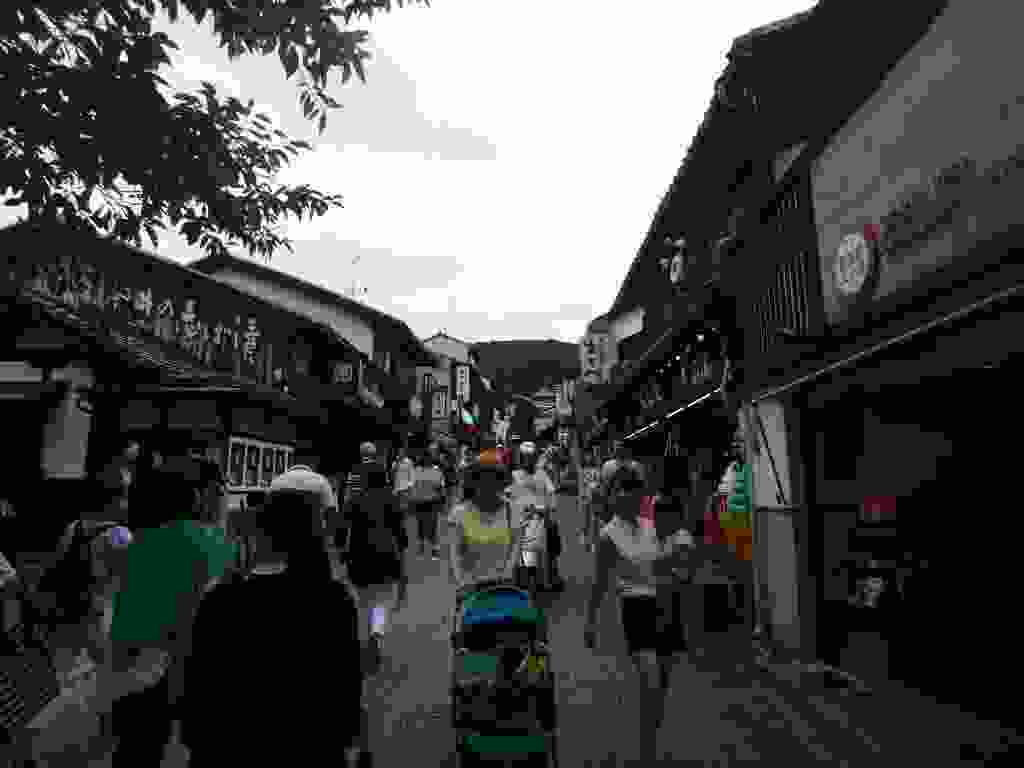
\includegraphics[width=\mywidth]{../wp-content/uploads/2015/08/P8196296-1024x768.jpg} } 
 \newline
 \newline
\centerline{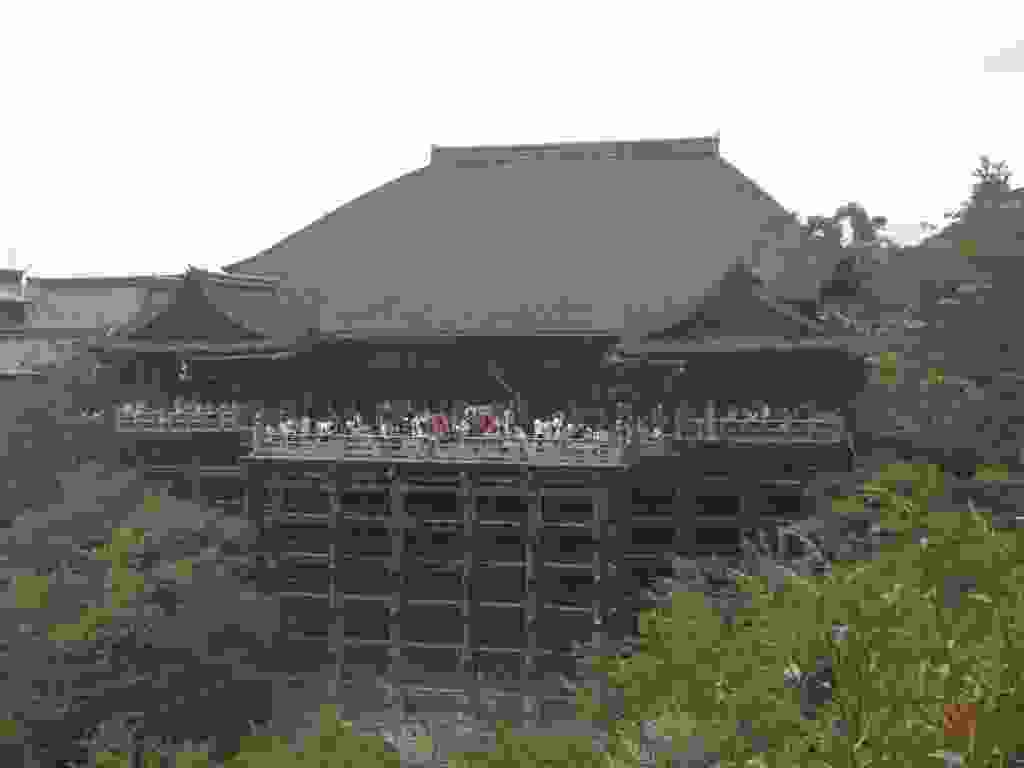
\includegraphics[width=\mywidth]{../wp-content/uploads/2015/08/P8196308-1024x768.jpg} } 
 \newline
 Temple Nishi Hongan-ji, le seul de ceux que j'ai vu qui n'était pas seulement touristique, avec des moines dedans \newline
 \newline
\centerline{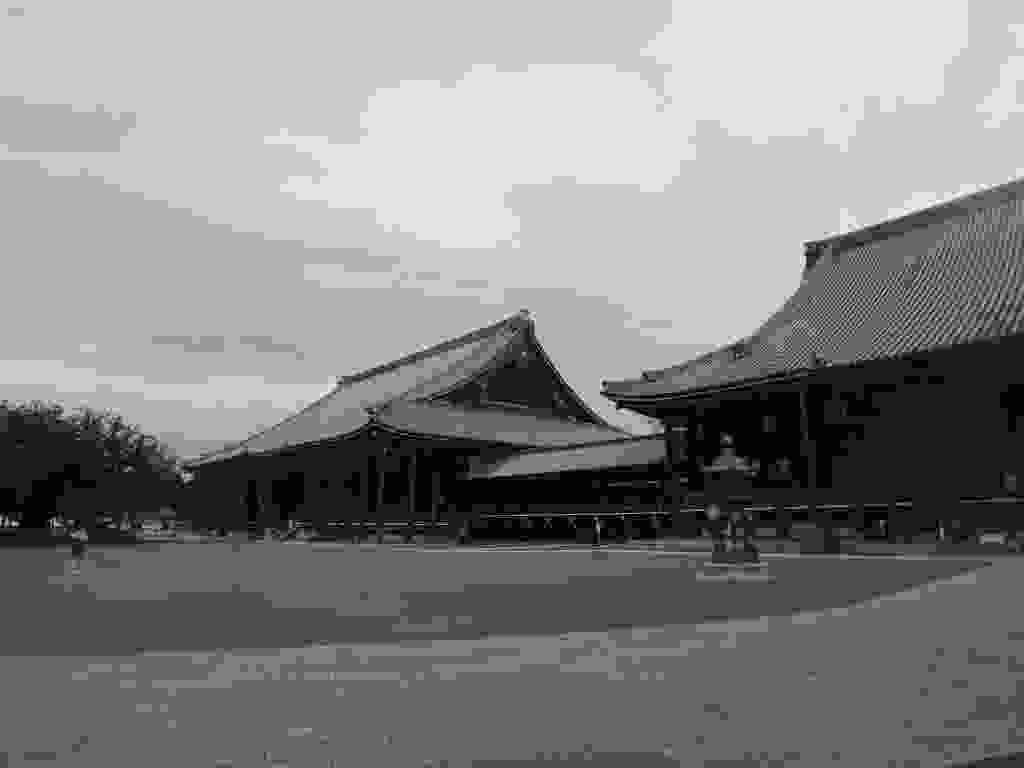
\includegraphics[width=\mywidth]{../wp-content/uploads/2015/08/P8196320-1024x768.jpg} } 
 \newline
 \newline
\centerline{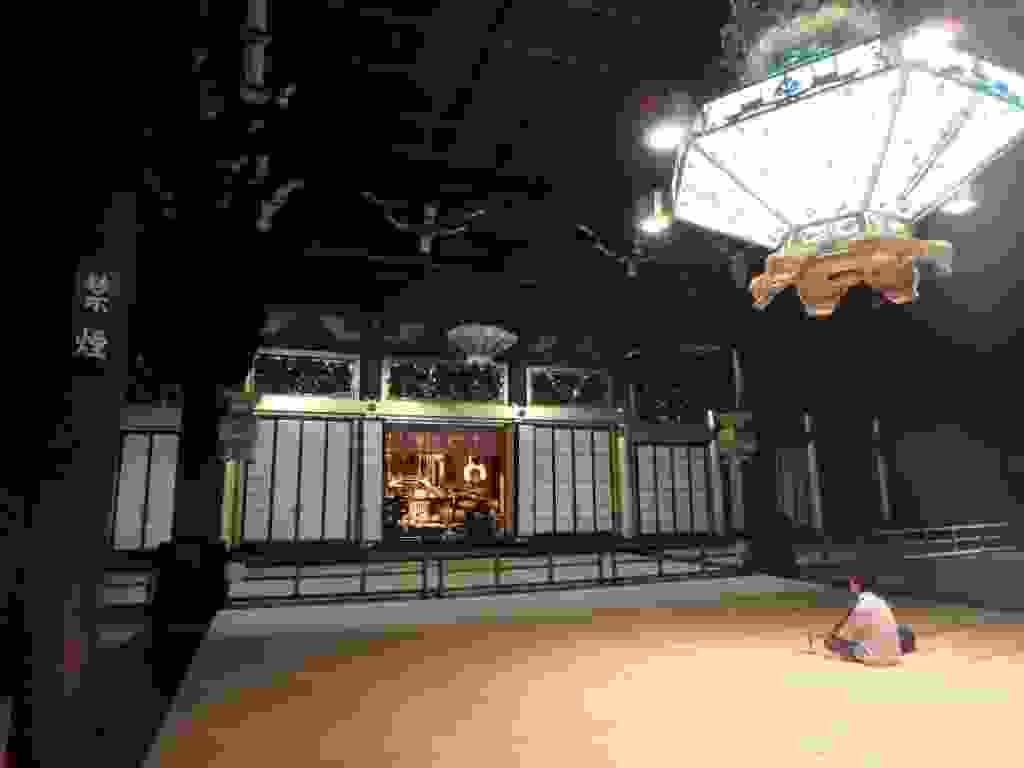
\includegraphics[width=\mywidth]{../wp-content/uploads/2015/08/P8196322-1024x768.jpg} } 
 \newline
 Le vieux quartier de Gion \newline
 \newline
\centerline{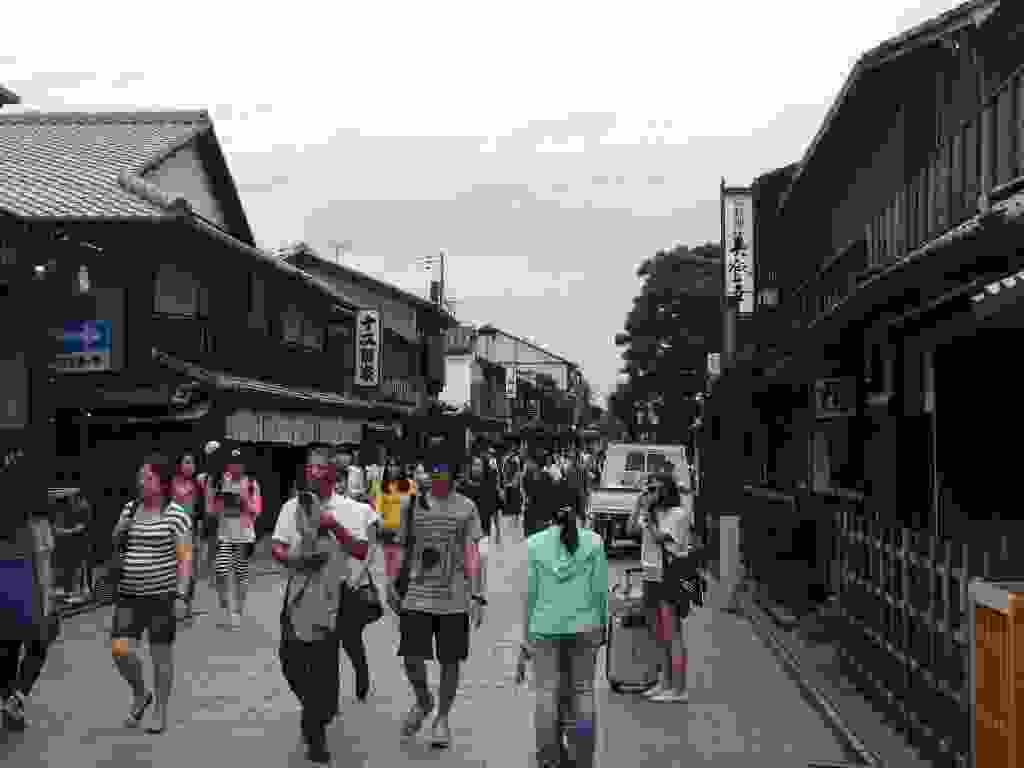
\includegraphics[width=\mywidth]{../wp-content/uploads/2015/08/P8196314-1024x768.jpg} } 
 \newline
 Kyoto Station, un peu de modernité \newline
 \newline
\centerline{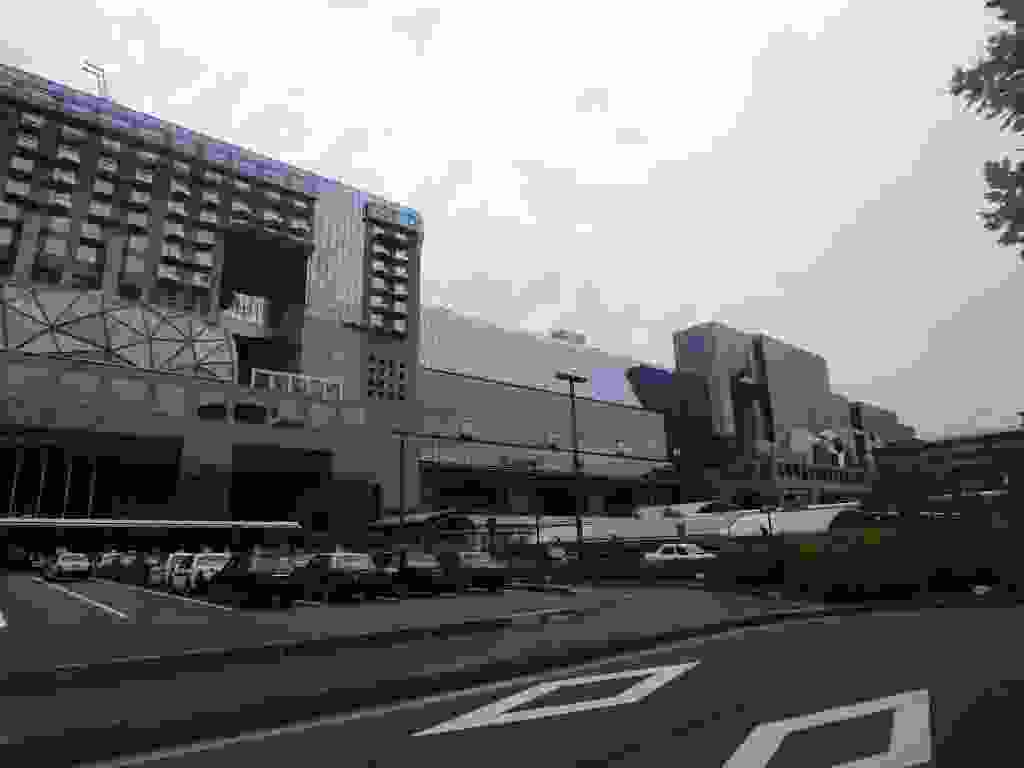
\includegraphics[width=\mywidth]{../wp-content/uploads/2015/08/P8196315-1024x768.jpg} } 
 \newline
 Parking à vélo dans un centre commercial \newline
 \newline
\centerline{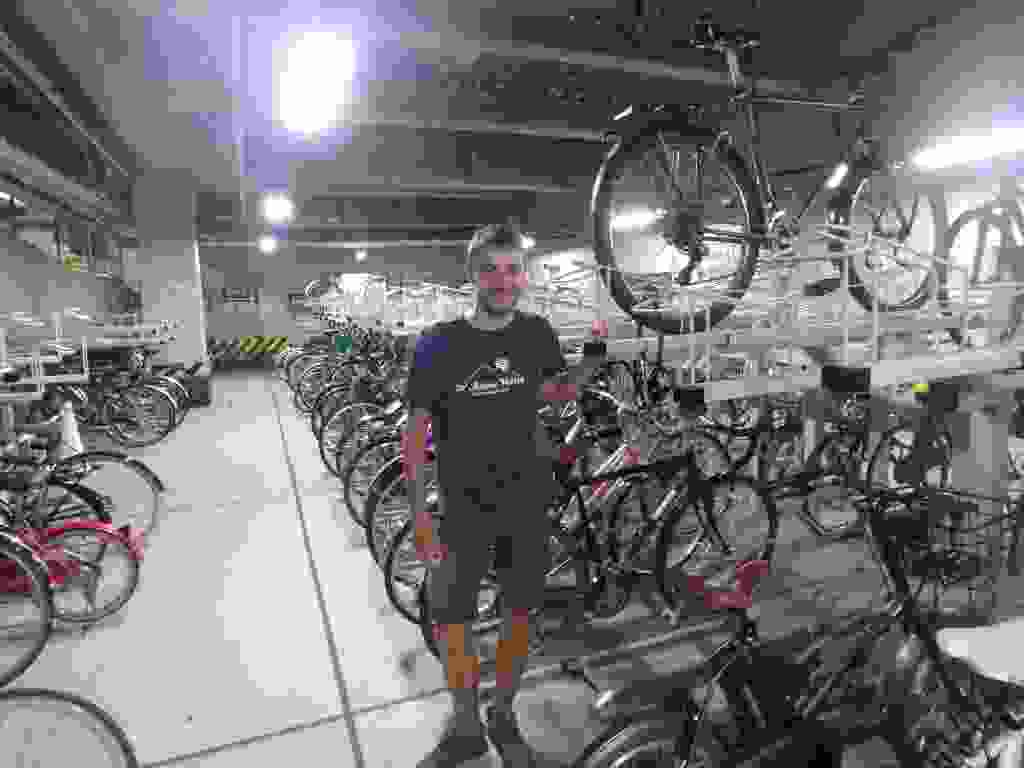
\includegraphics[width=\mywidth]{../wp-content/uploads/2015/08/P8196327-1024x768.jpg} } 
 \newline
 Un immense magasin de produits électroniques, finalement c'est tout petit la fnac. \newline
 \newline
\centerline{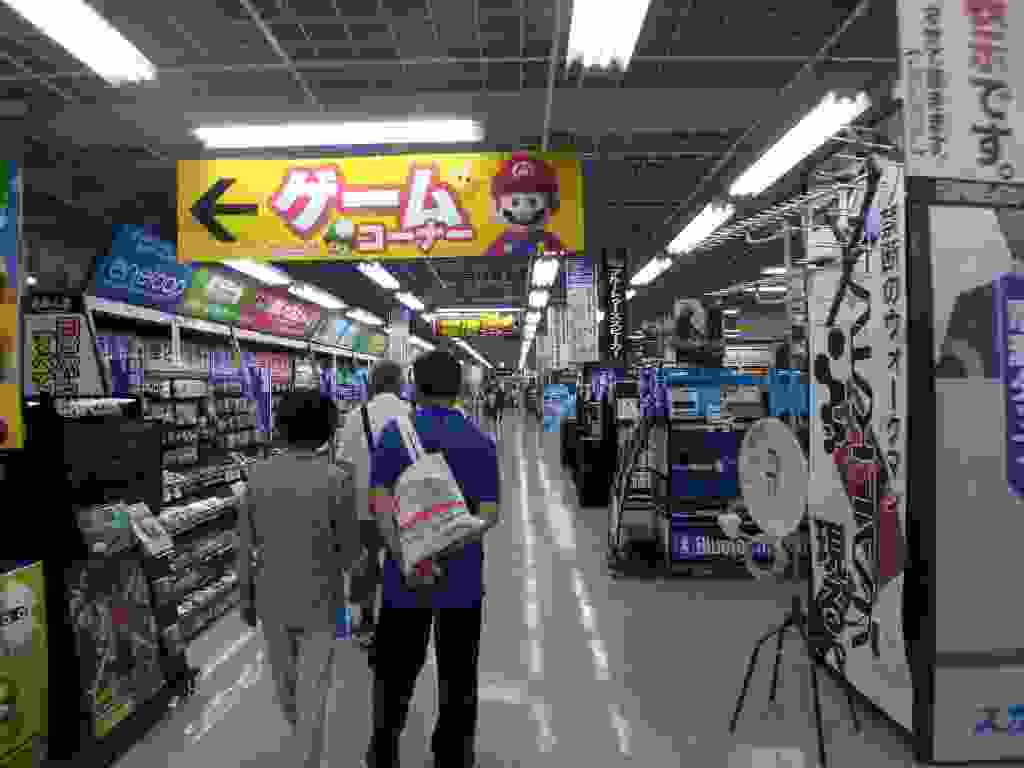
\includegraphics[width=\mywidth]{../wp-content/uploads/2015/08/P8196329-1024x768.jpg} } 
 \newline

\newpage
 
